\newpage
\section{Launch Phase}
\subsection{General Analysis}
	\subsubsection{Requirements	 Analysis}
		Put in description of the requirements... \textbf{JESUS}
		\begin{itemize}
			\item Functional Requirements ("system shall do 'requirement' ")
			\item Non-functional Requirements ("system shall be 'requirement' ")
			\item Behavioural Requirements ("how the system shall react")
			\item Performance Requirements ("how well does it have to be done")
		\end{itemize}
		\begin{figure}[h!]		%Remember to put the h!, to not fuck the sections.
			\begin{centering}
				 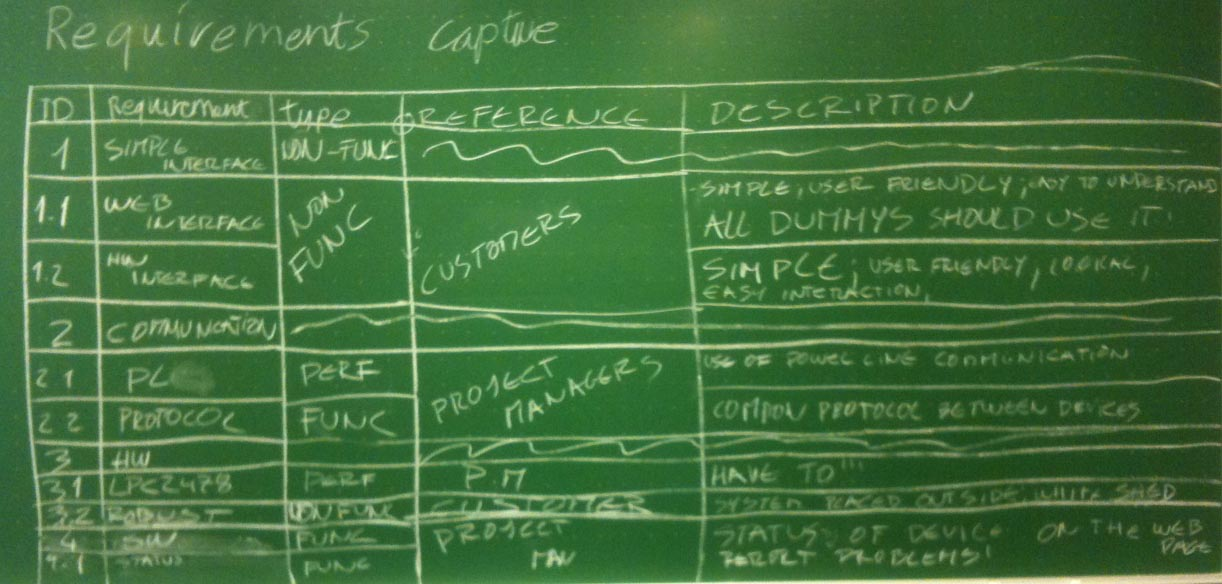
\includegraphics[width=1.0\textwidth]{images/requirement_capture.JPG}
		 		\caption{Design}
			 \end{centering}
		\end{figure}
	\subsubsection{Problem Domain Analysis}
			\paragraph{Block Diagram: Candidates in the system}
			\begin{itemize}
				\item \textbf{Consumers} Units that consumes power (e.g. light, washing machine, electric car)
				\item \textbf{Producers:} Modules that delivers energy to the hub (e.g. Wind-turbine, photovoltaic-cells)
				\item \textbf{Storage:} Modules that both consumes when the system over produces and "produces" (gives energy to the consumers) when needed. 
				\item \textbf{Temperature:} Unit that measures the outdoor temperature. If the temperature is too high or low it might damage the hardware.
				\item \textbf{Humidity:} Unit that measures the humidity where the system is places. If the humidity is too high.
			\end{itemize}
			\paragraph{Block Diagram: Events in the system}
				\begin{itemize}
					\item TemperatureBelowLimit
					\item TemperatureAboveLimit
					\item HumidityAboveLimit
					\item EnergyAboveLimit
					\item EnergyBelowLimit
					\item InitModule
					\item StartModule
					\item StopModule
					\item StandbyModule
				\end{itemize}
				\textbf{Table with all the above candidates and event combined:}
				\begin{table}[h!]
					\begin{tabular}{| r | c | c | c | c | c |}
					\hline
					~ & Consumers & Producers & Storage & Temp & Humidity \\ \hline
					TempBellowLimit & ~ & ~ & ~ & X & ~ \\ \hline
					TempAboveLimit & ~ & ~ & ~ & X & ~ \\ \hline
					HumidityAboveLimit & ~ & ~ & ~ & ~ & X \\ \hline
					InitModule & X & X & X & ~ & ~ \\ \hline
					StartModule & X & X & X & ~ & ~ \\ \hline
					StopModule & X & X & X & ~ & ~ \\ \hline
					StandbyModule & ~ & X & X & ~ & ~ \\ \hline
					EnergyAboveLimit & ~ & X & ~ & ~ & ~ \\ \hline
					EnergyBelowLimit & ~ & X & ~ & ~ & ~ \\
					\hline
					\end{tabular}
				\end{table}
			\newpage
			\paragraph{State Machine Diagrams}
				\textbf{Description of the different states:}
				\\ After the initialization of all peripherals connected to the hub, it enters \textit{Run Mode}.
				The system stays in Run Mode until event happens, e.g. temperature or humidity reaches their limits,
				a new module is connected, a module should be removed, the system is over-/underproduces, the log should be updated ect. 
				\\\textbf{Standby:}If the system overproduces (produces more energy than there is users for), it can standby some of the energy-producing modules.
				\\\textbf{Start:}Whenever a new module is connected it waits for the user to start up the module, either by using a start button on the hub or from the webpage.
				\\\textbf{Stop:}To securely disconnect a module, the user must use the disconnect button (on the module or from web) to make sure all data is saved.
				\\\textbf{Shut down:}If the system finds it self in a critical condition (temperature, humidity, communication problems) it shuts down it's connected modules,
							        tries to save all available data to the log. Then it sends an message (in form of mail) to the user with the problem where after the modules
							        powers off itself. 
				\\\textbf{Connect module:}At first the system checks if it has seen exactly that module before, if that is the case it updates variables from the database
									(uptime, produces etc.). If the module is new for the system, it creates it in the database and gives it an unique id.
				\\\textbf{Warning:}is sent if the system tries to send a submodule in standby- , start- or stop mode, but after a while it has not changed (timeout). 
							    After the timeout state, the system returns to run state. The system might also try to restart the device after a while.
				
			\begin{figure}[h!]		%Remember to put the h!, to not fuck the sections.
				\begin{centering}
					 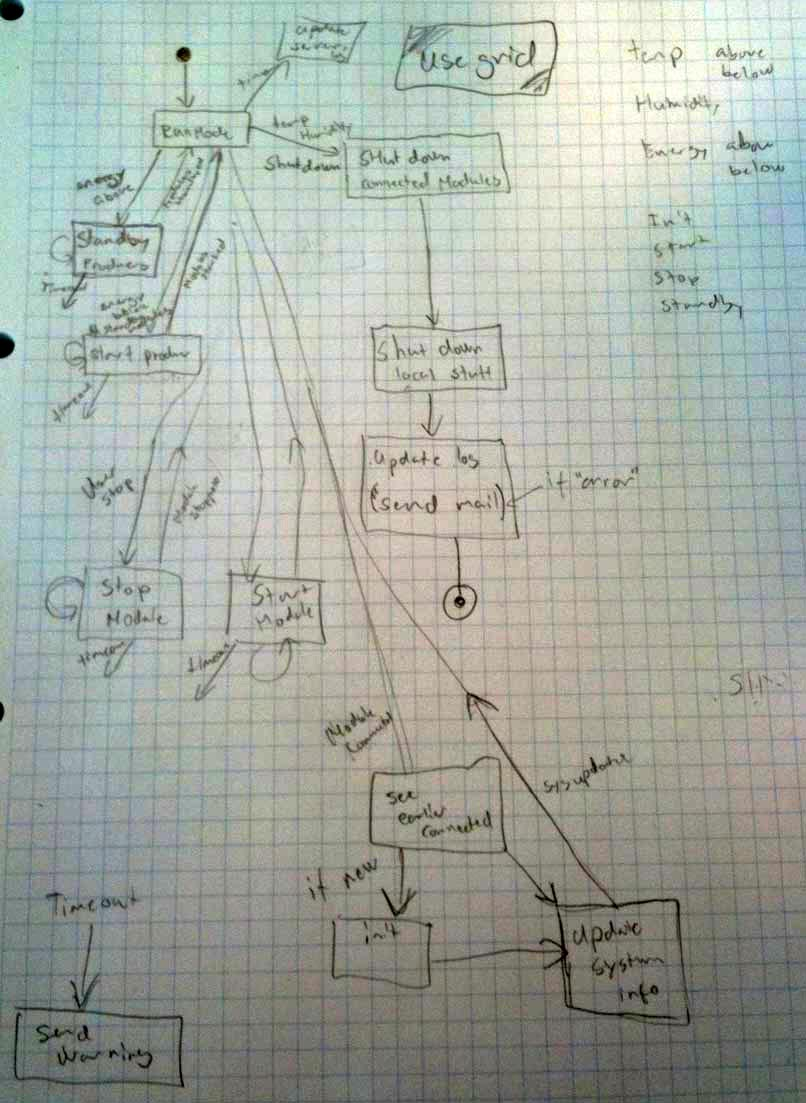
\includegraphics[width=0.5\textwidth]{images/statemachine.JPG}
		 			\caption{Statemachine}
			 	\end{centering}
			\end{figure}

	\subsubsection{Usage Domain Analysis}
		\begin{itemize}
			\item Use Cases - Put in diagrams of user + system (modules)
		\end{itemize}
	\subsubsection{Interface Analysis}
			Put in the comic book story!  \textbf{JESUS}
		\begin{itemize}
			\item User Interface Descriptions
				
			\item System Interface Descriptions
		\end{itemize}
	\subsubsection{Function Analysis}
	 \textbf{THIS}
		\begin{itemize}
			\item Recognise the direction of the device ( input, output, both ).
			\item Start / Stop slave devices from web interface or physical module ( Control over the connected modules ).
			\item Routes energy from the input to output ports.
			\item Control power status of slave modules.
			\item Log device data ( uptime of the port and power amount since connected ).
			\item More to add here...
		\end{itemize}
	\subsubsection{System Dynamics}
			Put in example from eudp: %eudp.dk/index.php/Sequence_Diagrams
			 \textbf{JESUS / DENNES}
		\begin{itemize}
			\item Communication Diagram
			\item Sequence Diagram
		\end{itemize}
	\subsubsection{General Analysis Specification}
		 \textbf{THIS}
\subsection{General Architecture Design}
	\subsubsection{Design Criteria}
		Write in what parts should be used (mostly off the shelf things).  \textbf{THIS}
	\subsubsection{Subsystem Design}
		\begin{itemize}
			\item Subsystem Architecture Diagram
			\item Detailed Block Diagrams
		\end{itemize}
	\subsubsection{Architecture Dynamics}
		Hubs communication with submodules
		\begin{itemize}
			\item Sequence Diagrams
		\end{itemize}
	\subsubsection{Architectural Specification and Constraints}
\subsection{Technical Platform}
	A lot of technical stuffs. 
	\subsubsection{Hardware Specifications}
	\subsubsection{Software Specifications}